\begin{center}
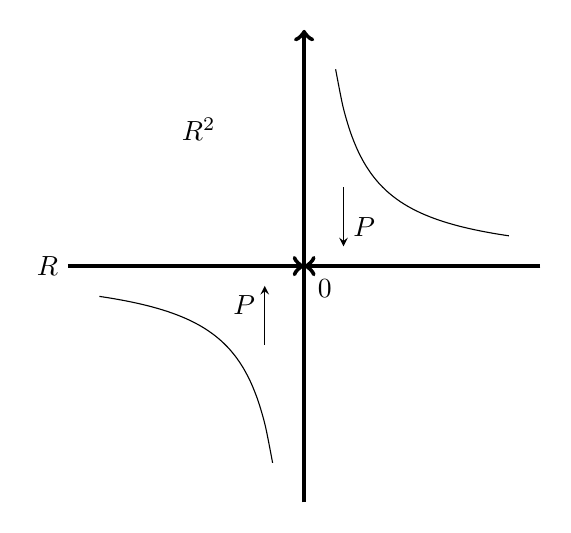
\begin{tikzpicture}
\draw[->, ultra thick] (0,3) -- (3,3);
\draw[->, ultra thick] (6,3) -- (3,3);
\draw[->, ultra thick] (3,0) -- (3,6);

\node[anchor=east] at (0, 3) {$\mathbb{R}$};
\node[anchor=north east] at (2, 5) {$\mathbb{R}^2$};
\node[anchor=north west] at (3.05,2.95) {$0$};

\draw[scale=1, domain=3.4:5.6, smooth, variable=\x, black] plot ({\x}, {1/(\x-3)+3});
\draw[scale=1, domain=0.4:2.6, smooth, variable=\x, black] plot ({\x}, {1/(\x-3)+3});

\draw [-stealth](3.5,4) -- (3.5,3.25) node[anchor=south west] {$P$};
\draw [-stealth](2.5,2) -- (2.5,2.75) node[anchor=north east] {$P$};

\end{tikzpicture}
\end{center}